\documentclass[tightenlines,twocolumn,prl,notitlepage,nofootinbib,preprintnumbers,longbibliography]{revtex4-1}
\usepackage{graphicx}
\usepackage{hyperref}
\hypersetup{colorlinks=true, linkcolor=blue, urlcolor=blue, citecolor=blue, final}
\usepackage{tabularx}
\usepackage{multirow}
\usepackage{array}
\usepackage[percent]{overpic}
\usepackage{float}
\usepackage[inline]{asymptote}
\usepackage{rotating}
\usepackage{epsfig}
\usepackage{xcolor}
\usepackage{amsmath}
\usepackage{amssymb}
\usepackage{bm}
\usepackage{pict2e}


\usepackage{tikz}
\usetikzlibrary{positioning}
\usetikzlibrary{matrix}
\usepackage[normalem]{ulem}
\usepackage{verbatim}

\begin{document}

\title{Enhancing Angular Sensitivity of Segmented Antineutrino Detectors for Reactor Monitoring Applications}

\author{Brian~C.~Crow}
\author{Max~A.~A.~Dornfest}
\author{John~G.~Learned}
\author{Jackson~D.~Seligman}
\author{Nathan~S.~Sibert}
\author{Jeffrey~G.~Yepez}
\affiliation{Department of Physics and Astronomy, University of Hawai'i at M\={a}noa}
\author{Viacheslav~A.~Li}
\affiliation{Lawrence Livermore National Laboratory}

\date{\today}



We should use this too:

\begin{figure}[ht]
    \begin{overpic}[width=1.0\linewidth]{fig/RAT_PAC_IBD_run_6_5_crop.png}
    
    \put(16.5,90){\color{white}\vector(0,-1){5}}
    \put(0,93){\fcolorbox{white}{white!30}{\parbox{70pt}{neutron capture ${\color{orange}n} \; {^6}\mathrm{Li} \to {^3}\mathrm{H}\;\; {^4}\mathrm{He}$}}}
    
    \put(67,45){\color{white}\vector(0,1){15}}
    \put(57,41){\fcolorbox{white}{white!30}{\parbox{50pt}{positron\\ annihilation ${\color{red}e^+} e^- \to {\color{green}\gamma} \; {\color{green}\gamma}$}}}

    \put(81,86){\color{white}\vector(0,-1){15}}
    \put(65,85){\fcolorbox{white}{white!30}{\parbox{70pt}{inverse $\beta$ decay $\bar\nu_e \; ^1\mathrm{H} \to {\color{red}e^+ } \;{\color{orange}n}$}}}
    \end{overpic}
    \caption{Rendering of RAT-PAC 2 IBD visualization. Positron track in red, neutron track --- orange, gamma-rays --- green, Cherenkov photons --- cyan. Scintillation light turned off for clarity. Cherenkov photons indicate the direction of the positron, which traveled from the top right to the bottom left in this perspective (neutrino, not shown, is from top right to bottom left.}
    \label{fig_RATPAC_IBD_visual}
\end{figure}

More Useful plots:

% Binning matrix - just use one. maybe 30 deg
\begin{figure*}[ht]
\centering
\begin{tabular}{ccc}
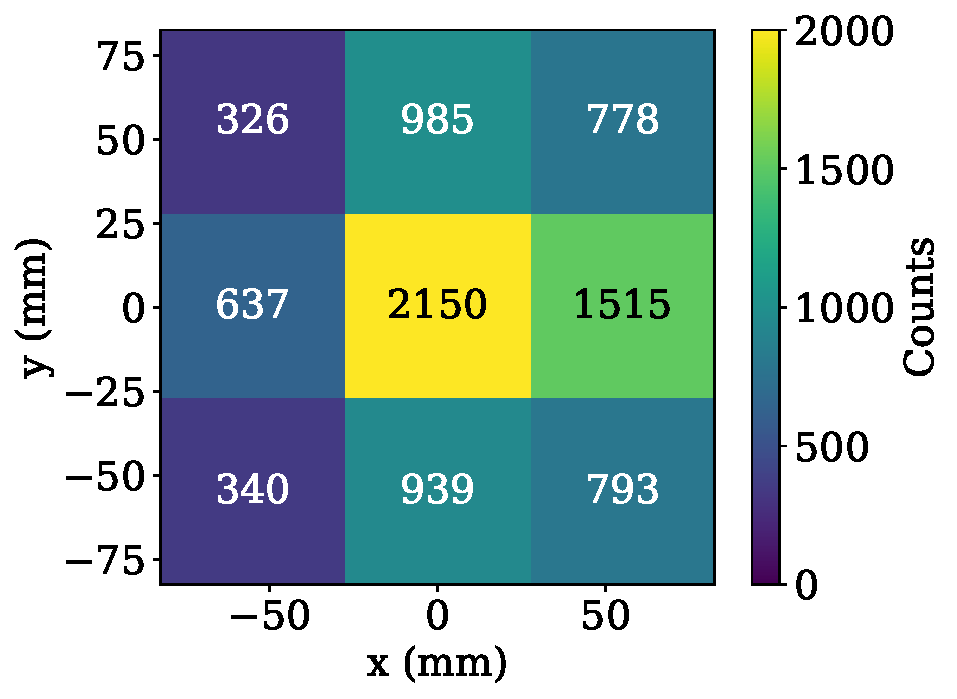
\includegraphics[width=0.32\linewidth]{fig/bin_dist_rot0_001wt.pdf}
&
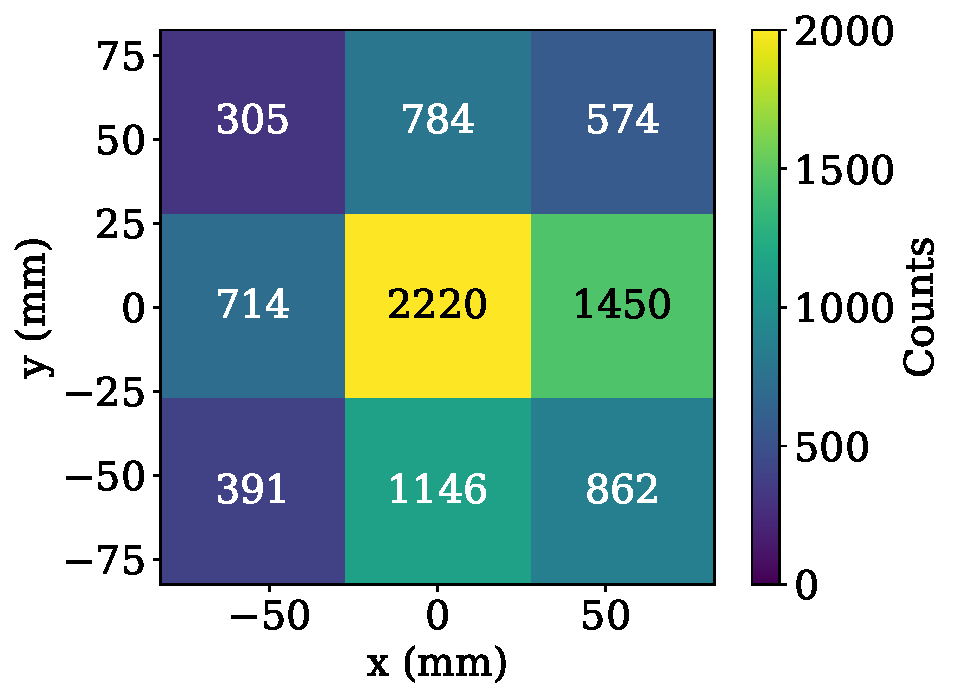
\includegraphics[width=0.32\linewidth]{fig/bin_dist_rot30_001wt.pdf}
&
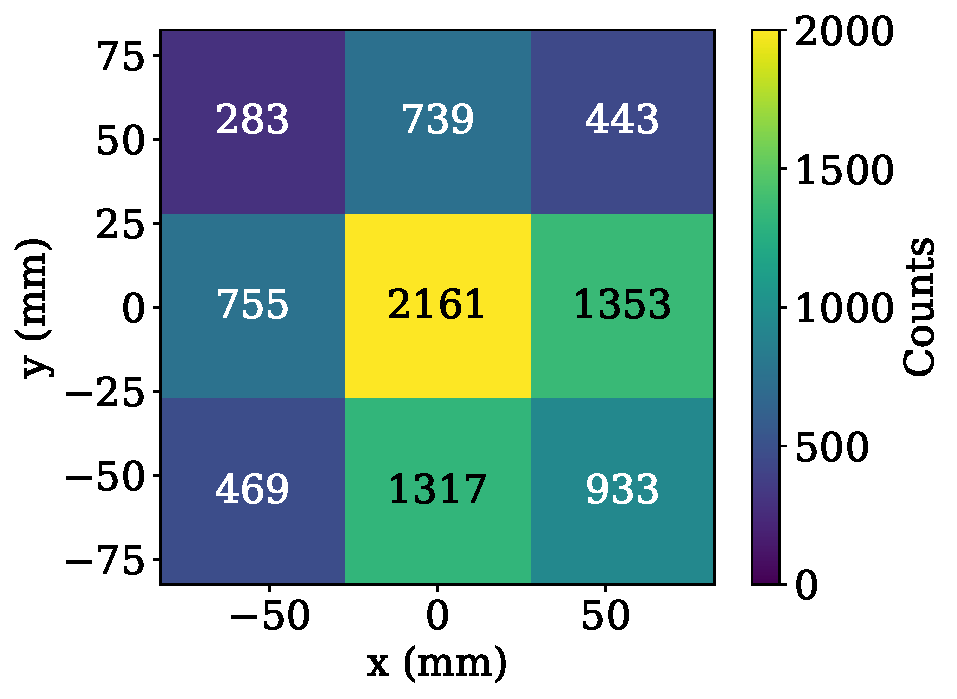
\includegraphics[width=0.32\linewidth]{fig/bin_dist_rot45_001wt.pdf} \\
\end{tabular}

    \begin{tabular}{>{\centering\arraybackslash}p{0.32\linewidth} >{\centering\arraybackslash}p{0.32\linewidth}>{\centering\arraybackslash}p{0.32\linewidth}}
        \makebox[0.32\linewidth][c]{%
            \begin{picture}(20,20)
                \put(-5,13){\color{black}\vector(1,0){20}} 
            \end{picture}
        }
        &
        \makebox[0.32\linewidth][c]{%
            \begin{picture}(20,20)
                \put(-3,17){\color{black}\vector(2,-1){18}} 
            \end{picture}
        }
 &
        \makebox[0.32\linewidth][c]{%
            \begin{picture}(20,20)
                \put(-1,19){\color{black}\vector(1,-1){14}} 
            \end{picture}
        }        \\
\hspace{-0.5cm}$\vartheta_\nu = 0^\circ$ & $\vartheta_\nu = -30^\circ$ & $\vartheta_\nu = -45^\circ$ 
    \end{tabular}
    \caption{Examples of binning distributions for incoming angles $\vartheta_\nu=0^\circ,-30^\circ,-45^\circ$, 0.1\%\ ${}^6$Li-doped. The direction of antineutrinos is indicated by the arrows below the plots.}
    \label{fig:trackplot3dratpac_001wt}
\end{figure*}

% FND fit plot
\begin{figure}[ht]
    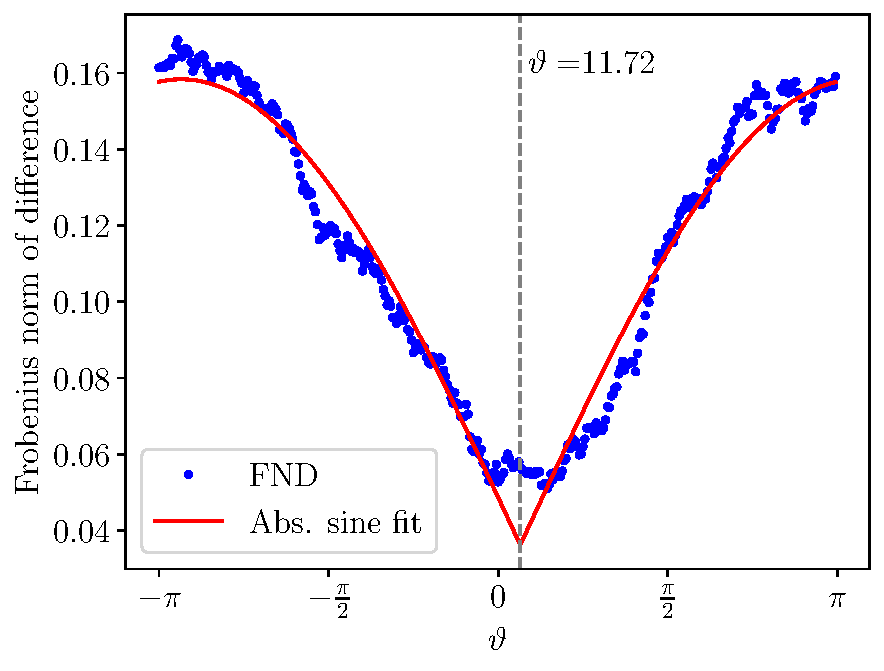
\includegraphics[width=1\linewidth]{fig/FND_plot.pdf}
    \caption{Frobenius norm of the difference between an artificial reference dataset produced for a true angle of $\vartheta_{true} = 0^\circ$ and the datasets for all angles within $\pm\pi$ radians from either side of the reference angle. Uses $50 \,\text{mm}$ segment size and $n=1000$. The FND of the neutron capture distribution data was fit with an absolute value of sine function as prescribed by the theoretical proof for the direction algorithm \cite{10.1063/5.0315079}.}
    \label{fig:CFND_1iteration}
\end{figure}
\begin{figure}[ht]
        \setlength{\unitlength}{.1\linewidth}
\begin{picture}(10,5)
        \multiput(5,0)(.5,0){9}{\color{black}\line(0,1){4}} 
        \multiput(5,0)(0,0.5){9}{\color{black}\line(1,0){4}} 

        \multiput(5,4)(.5,0){9}{\color{black}\line(1,1){1}} 
        \multiput(9,0)(0,.5){9}{\color{black}\line(1,1){1}} 

        \put(10,1){\line(0,1){4}}
        \put(6,5){\line(1,0){4}}

        
          \thicklines
        \multiput(6.5, 2.50)(.025,0){20}{\color{black}\line(0,1){0.5}} 
        \multiput(0, 5)(.025,0){20}{\color{black}\line(0,-1){0.5}} 
        
        \multiput(6, 1.50)(.025,0){20}{\color{gray}\line(0,1){0.5}} 
        \multiput(0, 4.25)(.025,0){20}{\color{gray}\line(0,-1){0.5}} 
          \thinlines

        \put(0.8,4.7){prompt segment}
        \put(0.8,3.9){delayed segment}


        \put(1,1){\vector(-1,-1){1}} 
        \put(1,1){\vector(0,1){2}} 
        \put(1,1){\vector(1,0){2}} 

        \put(1,1){\vector(2,1){2}} 
        \put(1,1){\arc[0,26]{1}} 
        \put(1,1){\arc[0,26]{.95}} 

        
        \put(0,0.3){$z$}
        \put(0.7,2.8){$y$}
        \put(2.8,.7){$x$}
        \put(2.7,2){$\nu$}
        
       \put(6.75,-0.1){\color{black!90}\vector(0,1){4.7}} 
        \multiput(6.7,0.)(0,.25){16}{\color{blue}\line(1,0){0.1}}
        \put(4.8,2.75){\color{black!90}\vector(1,0){4.8}} 
        \multiput(5,2.7)(.25,0){16}{\color{blue}\line(0,1){0.1}} 

        \put(6.8,4.55){\color{black}$y'$}
        \put(9.2,2.4){\color{black}$x'$}
        \put(5.85,2.1){\color{black}$\theta_n^i$}


        \put(6.75,2.75){\color{blue}\arc[0,245]{0.65}} 
        \put(6.75,2.75){\color{blue}\vector(-1,-2){0.5}} 

        
        \multiput(3.5, 0.5)(0,1){4}{\color{black}\vector(2,1){1}} 
        
       \put(2,0){neutrino wind} 
        \put(2.2,1.2){$\vartheta_\nu$}
\end{picture}
        \caption{Diagram explaining the prompt-delayed segment geometry, as well as neutrino and axes orientation.
        In this work we assume that neutrino ``wind'' is in $xy$ plane, at an angle $\nu$ with the $x$ axis.
        The prompt and delayed segment in this diagram shown for illustrative purposes; the actual separation depends on the segment size --- for large segments, prompt and delayed events would happen in the same segment. It is also illustrated that capture is not necessarily aligned with the neutrino beam (only on average it is the case as discussed in this paper).
        To study the angular dependence we vary the angle of neutrino with respect to the detector's $x$ and $y$ axes (i.e. rotation of the detector along $z$ axis).}
        \label{fig:phi_def}
\end{figure}

Results section:

% Fig 3 from the paper, and money plot from paper A
\begin{figure}[ht]
    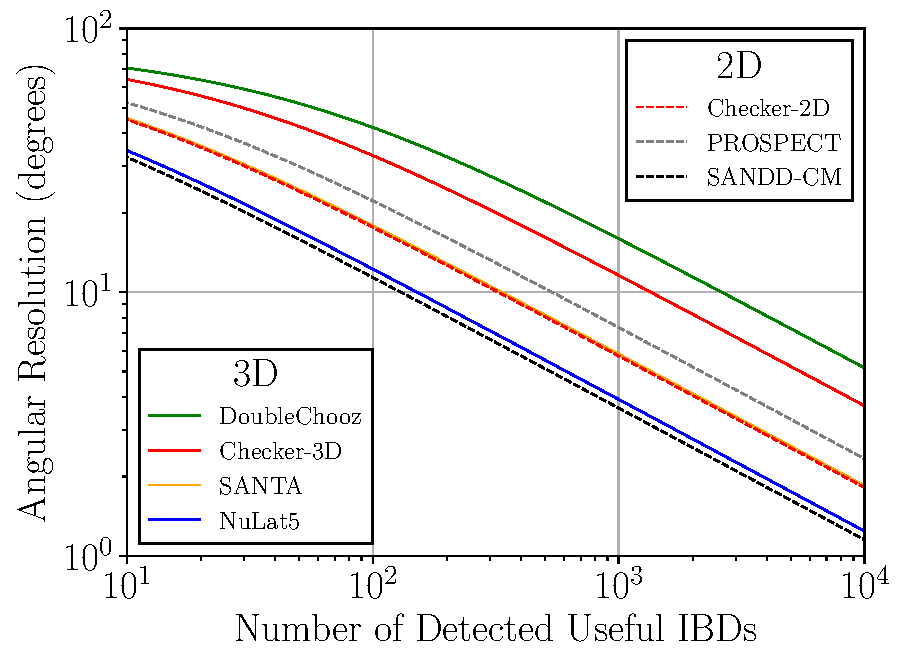
\includegraphics[width=1\linewidth]{fig/angular_resolution_analytic_ylog_PackFactor_v2Useful.pdf}
    \caption{Angular uncertainty calculated using the conventional ``Chooz" approach. A selected number of segmented detectors along with Chooz is highlighted. Useful IBD events are those that have prompt and delayed signals in separate segments. This result is taken from our previous study~\cite{Duvall:2024cae}.}
    \label{fig_old_method}
\end{figure}

% Fig 13 & money plot from paper B
\begin{figure}[ht]
    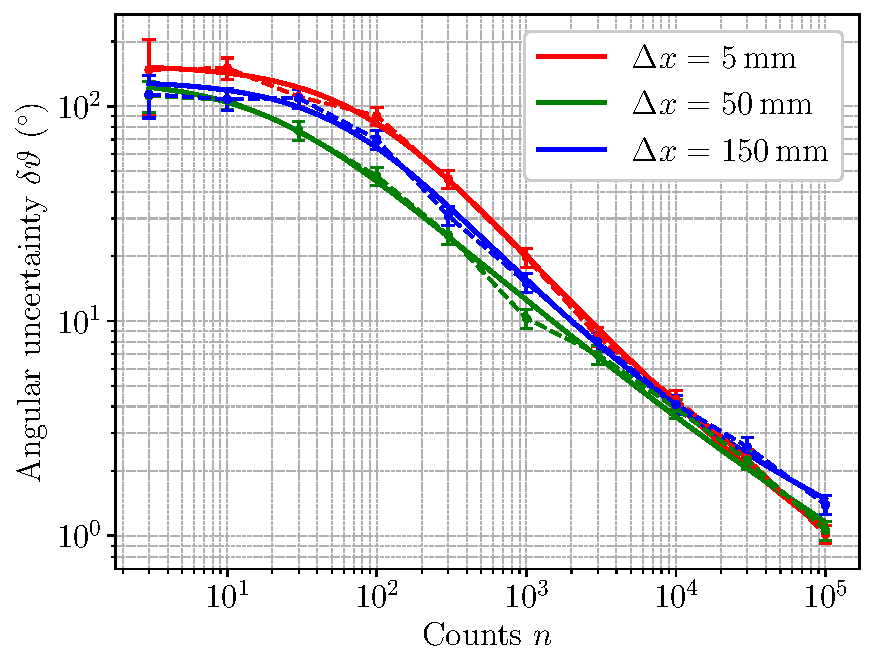
\includegraphics[width=1\linewidth]{fig/parallel/06_money_plot_fit_arctan_log_4p.pdf}
    \caption{Angular uncertainty plot comparing the performance of three different square segment sizes: 5 mm, 50 mm and 150 mm. Notice that the smallest segment size begins to perform better than the other two for higher counts. Smaller segment sizes outperform larger ones for higher counts simply due to superior resolution.}
    \label{fig:POI_segsize_uncert}
\end{figure}

\end{document}